\documentclass[a4paper, 10pt]{article}
\usepackage{fullpage} % changes the margin
\usepackage[english]{babel}
\usepackage[utf8]{inputenc}
\usepackage{hyperref}
\usepackage{xcolor}
\usepackage{graphicx}
\usepackage{array}
\usepackage{float}
\usepackage{longtable}
\usepackage[bottom]{footmisc}
\usepackage{cite}
\usepackage{parskip}
\usepackage{subcaption}
\usepackage{amssymb}
\usepackage{amsmath}
\usepackage{listings}
\usepackage[nocenter]{qtree}
\usepackage{tree-dvips}

\hypersetup{
	colorlinks=true,       % false: boxed links; true: colored links
	linkcolor=blue,        % color of internal links
	citecolor=blue,        % color of links to bibliography
	filecolor=magenta,     % color of file links
	urlcolor=blue
}

%\setlength{\parindent}{0cm}
\newcommand{\code}[1]{\texttt{#1}}
\newcommand{\suchthat}[0]{\hspace{1mm}|\hspace{1mm}}
\renewcommand{\arraystretch}{1.4}
\definecolor{statement}{gray}{0.5}

\graphicspath{{img/}}

\begin{document}

\noindent
\begin{flushright}
    \large\textbf{Miguel Alcón Doganoc} \\
    Algorithms for VLSI \\
    \today
\end{flushright}

\noindent
{\huge{\textbf{Exercises on physical design}}}

\section{Quadratic placement}
{\color{statement} 
Show the two linear system of equations for the x and y coordinates.
}

Our system of equations is
\[
     AX - b_x = 0\text{, and } AY - b_y = 0
\]
where
\[
    A = \begin{bmatrix}
        3 & 0 & -1 & -1 \\
        0 & 5 & -1 & 1 \\
        -1 & -1 & 4 & 0 \\
        -1 & -1 & 0 & 4
    \end{bmatrix}\hspace{3mm}
    X = \begin{bmatrix}
        X_a \\
        X_b \\
        X_c \\
        X_d \\
    \end{bmatrix}\hspace{3mm}
    b_x = \begin{bmatrix}
        5 & 6 & 5 & 10
    \end{bmatrix}\hspace{3mm}
    Y = \begin{bmatrix}
        Y_a \\
        Y_b \\
        Y_c \\
        Y_d
    \end{bmatrix}  \hspace{3mm}
    b_y = \begin{bmatrix}
        0 & 12 & 2 & 5
    \end{bmatrix}
\]
So, the final systems are
\[
    \begin{cases}
        3 X_a - X_c - X_d - 5 = 0  \\
        5 X_b - X_c - X_d - 6 = 0 \\
        - X_a - X_b + 4 X_c - 5 = 0 \\
        - X_a - X_b + 4X_d - 10 = 0 \\
    \end{cases}\hspace{3mm}
    \begin{cases}
        3 Y_a - Y_c - Y_d = 0  \\
        5 Y_b - Y_c - Y_d - 12 = 0 \\
        - Y_a - Y_b + 4 Y_c - 2 = 0 \\
        - Y_a - Y_b + 4Y_d - 5 = 0 \\
    \end{cases}
\]
{\color{statement} 
Solve the systems of equations and draw the final solution in a 2D plot.
}

The final solution is
\[
    a = (\frac{177}{44},\frac{59}{44})\hspace{8mm}b = (\frac{115}{44},\frac{141}{44})\hspace{8mm}c = (\frac{32}{11},\frac{18}{11})\hspace{8mm}d = (\frac{183}{41},\frac{105}{44})    
\]

\begin{figure}[htbp]
    \centering
    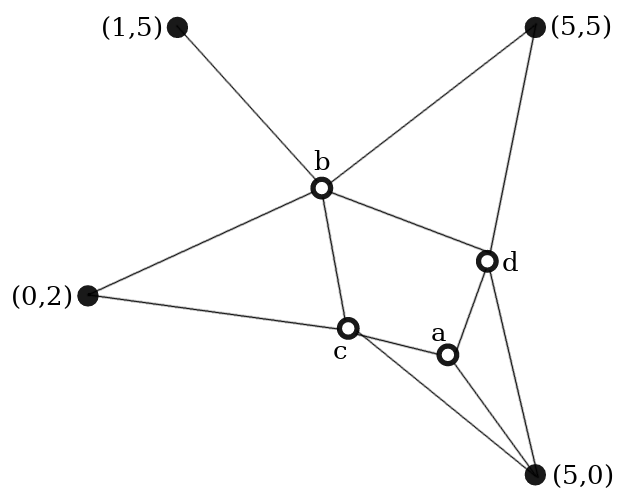
\includegraphics[width=0.5\linewidth]{1_qplacement.png}
    \caption{2D plot of the solution}
\end{figure}
\newpage
\section{Channel Routing}
{\color{statement} Draw the vertical constraint graph (VCG) without splitting the nets. Determine the zone representation for the nets. Draw the vertical constraint graph with net splitting.}
\begin{figure}[htbp]
    \centering
    \begin{subfigure}{0.32\textwidth}
        \centering
        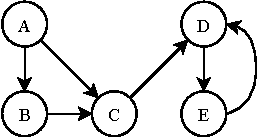
\includegraphics[width=\linewidth]{2_vcg.pdf}
        \caption{VCG without splitting}
        \label{}
    \end{subfigure}
    \hfill
    \begin{subfigure}{0.22\textwidth}
        \centering
        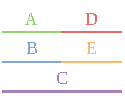
\includegraphics[width=\linewidth]{2_zr.pdf}
        \caption{Zone representation}
        \label{}
    \end{subfigure}
    \hfill
    \begin{subfigure}{0.32\textwidth}
        \centering
        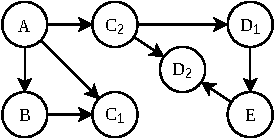
\includegraphics[width=\linewidth]{2_vcg_split.pdf}
        \caption{VCG without splitting}
        \label{}
    \end{subfigure}
\end{figure}


{\color{statement} Find the minimum number of required tracks with net splitting and without net splitting.}

Since without net splitting nodes $D$ and $E$ creates a loop in the VCG, it is impossible to route this channel.  With net splitting, I found the number of tracks after applying the Dogleg Left-Edge algorithm, which is 5. 

{\color{statement} Use the Dogleg Left-Edge algorithm to route this channel. For each track, state which nets are assigned. Draw the final routed channel.}

The assignment of nets to tracks is specified at the right of the route diagram.
\begin{figure}[H]
    \centering
    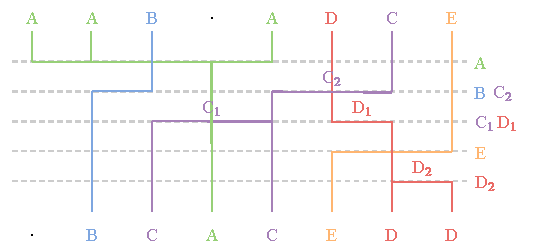
\includegraphics[width=1\linewidth]{2_route.pdf}
    \caption{Final routed channel}
\end{figure}
\newpage
\section{Slicing Floorplan}
{\color{statement} Find the smallest bounding box that can accommodate the slicing floorplan assuming that blocks can be rotated by 90º. Show the shape functions at each node of the tree and the final floorplan.}

\begin{figure}[H]
    \centering
    \begin{subfigure}{0.5\textwidth}
        \centering
        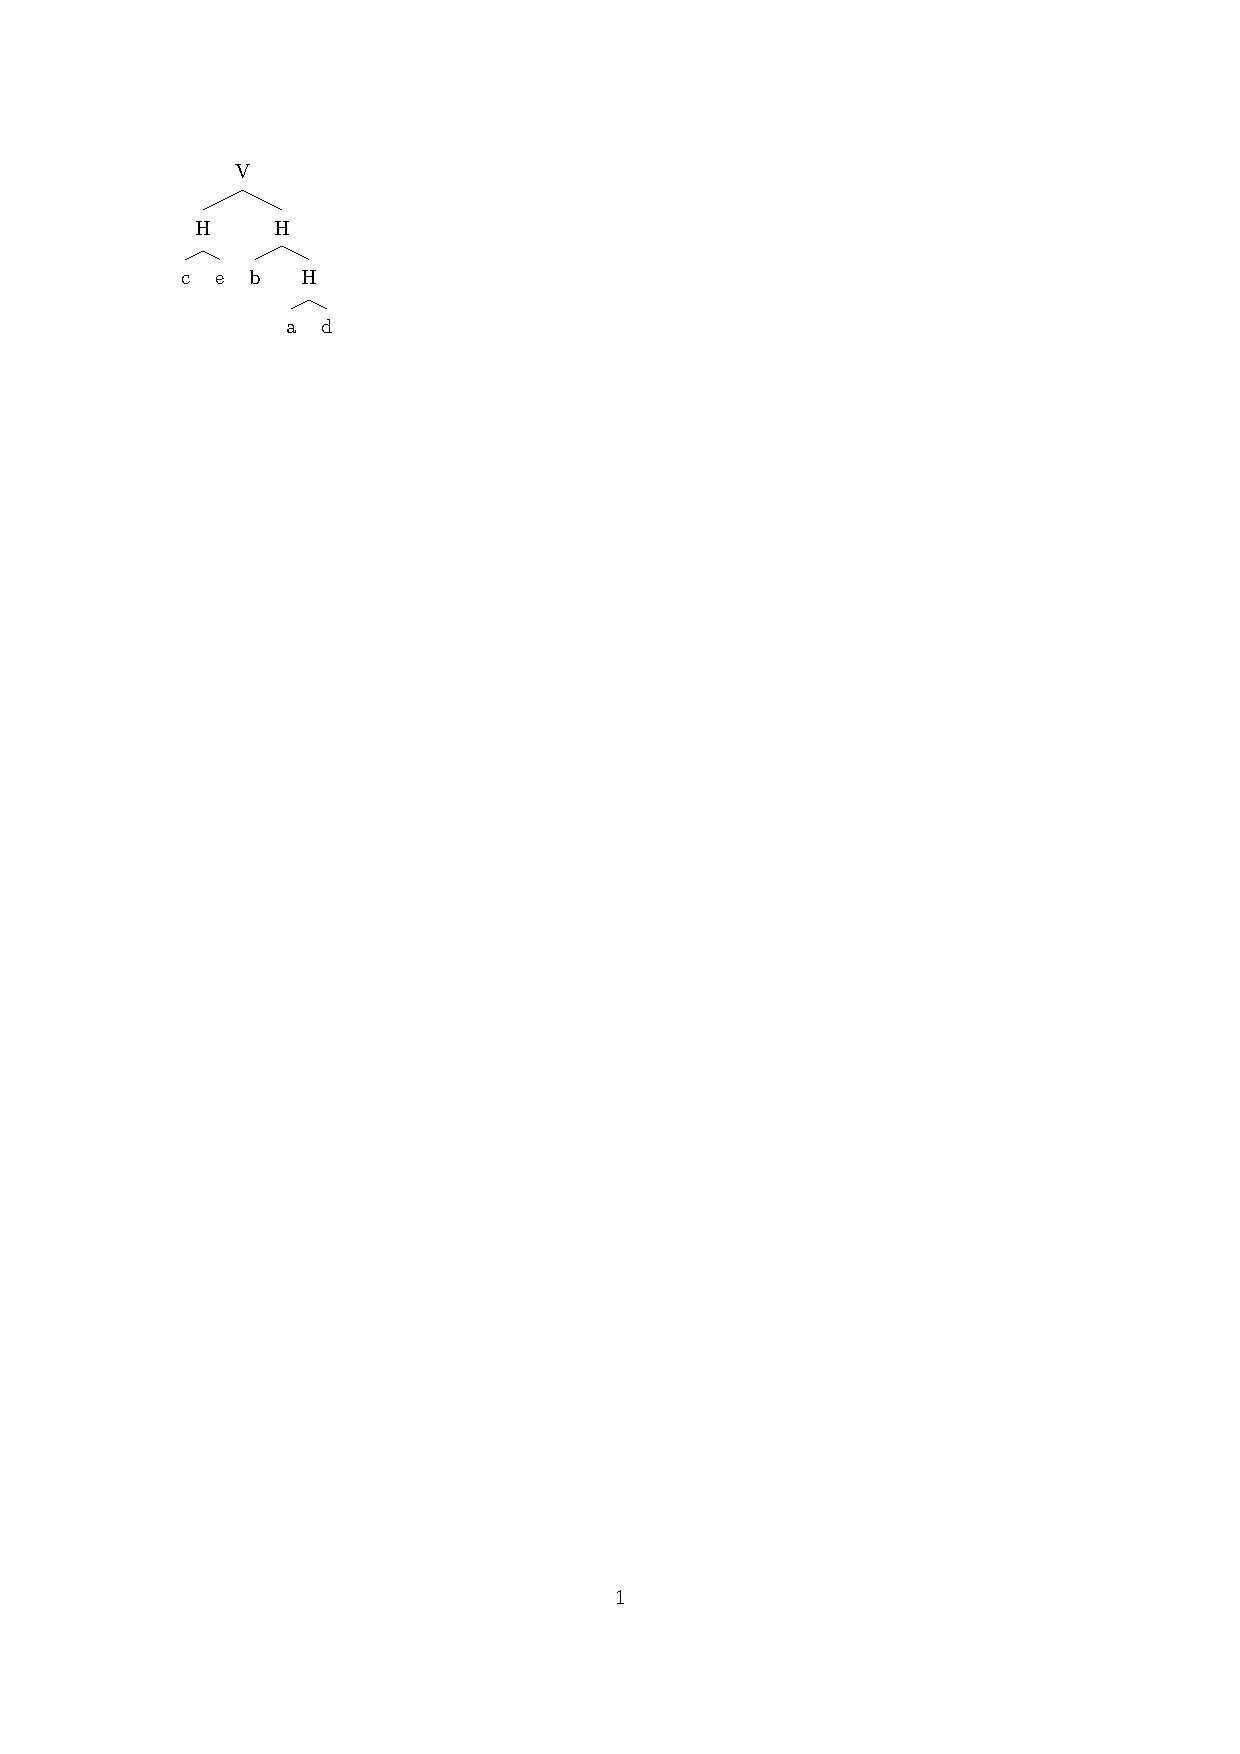
\includegraphics[trim=50 670 400 75,clip,width=1\linewidth]{tree1.pdf}
        \caption{Initial floorplan tree}
        \label{}
    \end{subfigure}
    \hspace{10mm}
    \begin{subfigure}{0.4\textwidth}
        \centering
        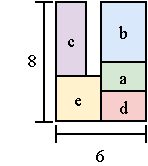
\includegraphics[trim=13 0 0 0,clip,width=0.6\linewidth]{3_floorplan1.pdf}
        \caption{Floorplan and bounding box}
        \label{}
    \end{subfigure}
\end{figure}



\begin{figure}[H]
    \centering
    \begin{subfigure}{0.35\textwidth}
        \centering
        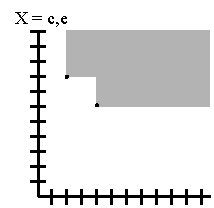
\includegraphics[width=\linewidth]{3_sfx.pdf}
    \end{subfigure}
    \hfill
    \begin{subfigure}{0.35\textwidth}
        \centering
        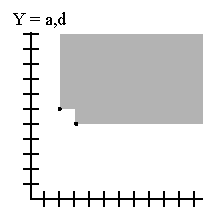
\includegraphics[width=\linewidth]{3_sfy.pdf}
    \end{subfigure}
    \begin{subfigure}{0.35\textwidth}
        \centering
        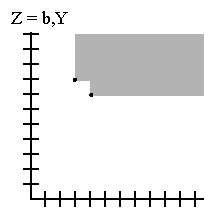
\includegraphics[width=\linewidth]{3_sfz.pdf}
    \end{subfigure}
    \hfill
    \begin{subfigure}{0.35\textwidth}
        \centering
        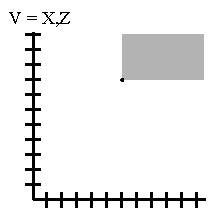
\includegraphics[width=\linewidth]{3_sfv.pdf}
    \end{subfigure}
    \caption{Shape functions}
\end{figure}

\newpage

{\color{statement} Find another slicing tree that can give a smaller floorplan. Draw the new floorplan.}

\begin{figure}[H]
    \centering
    \begin{subfigure}{0.52\textwidth}
        \centering
        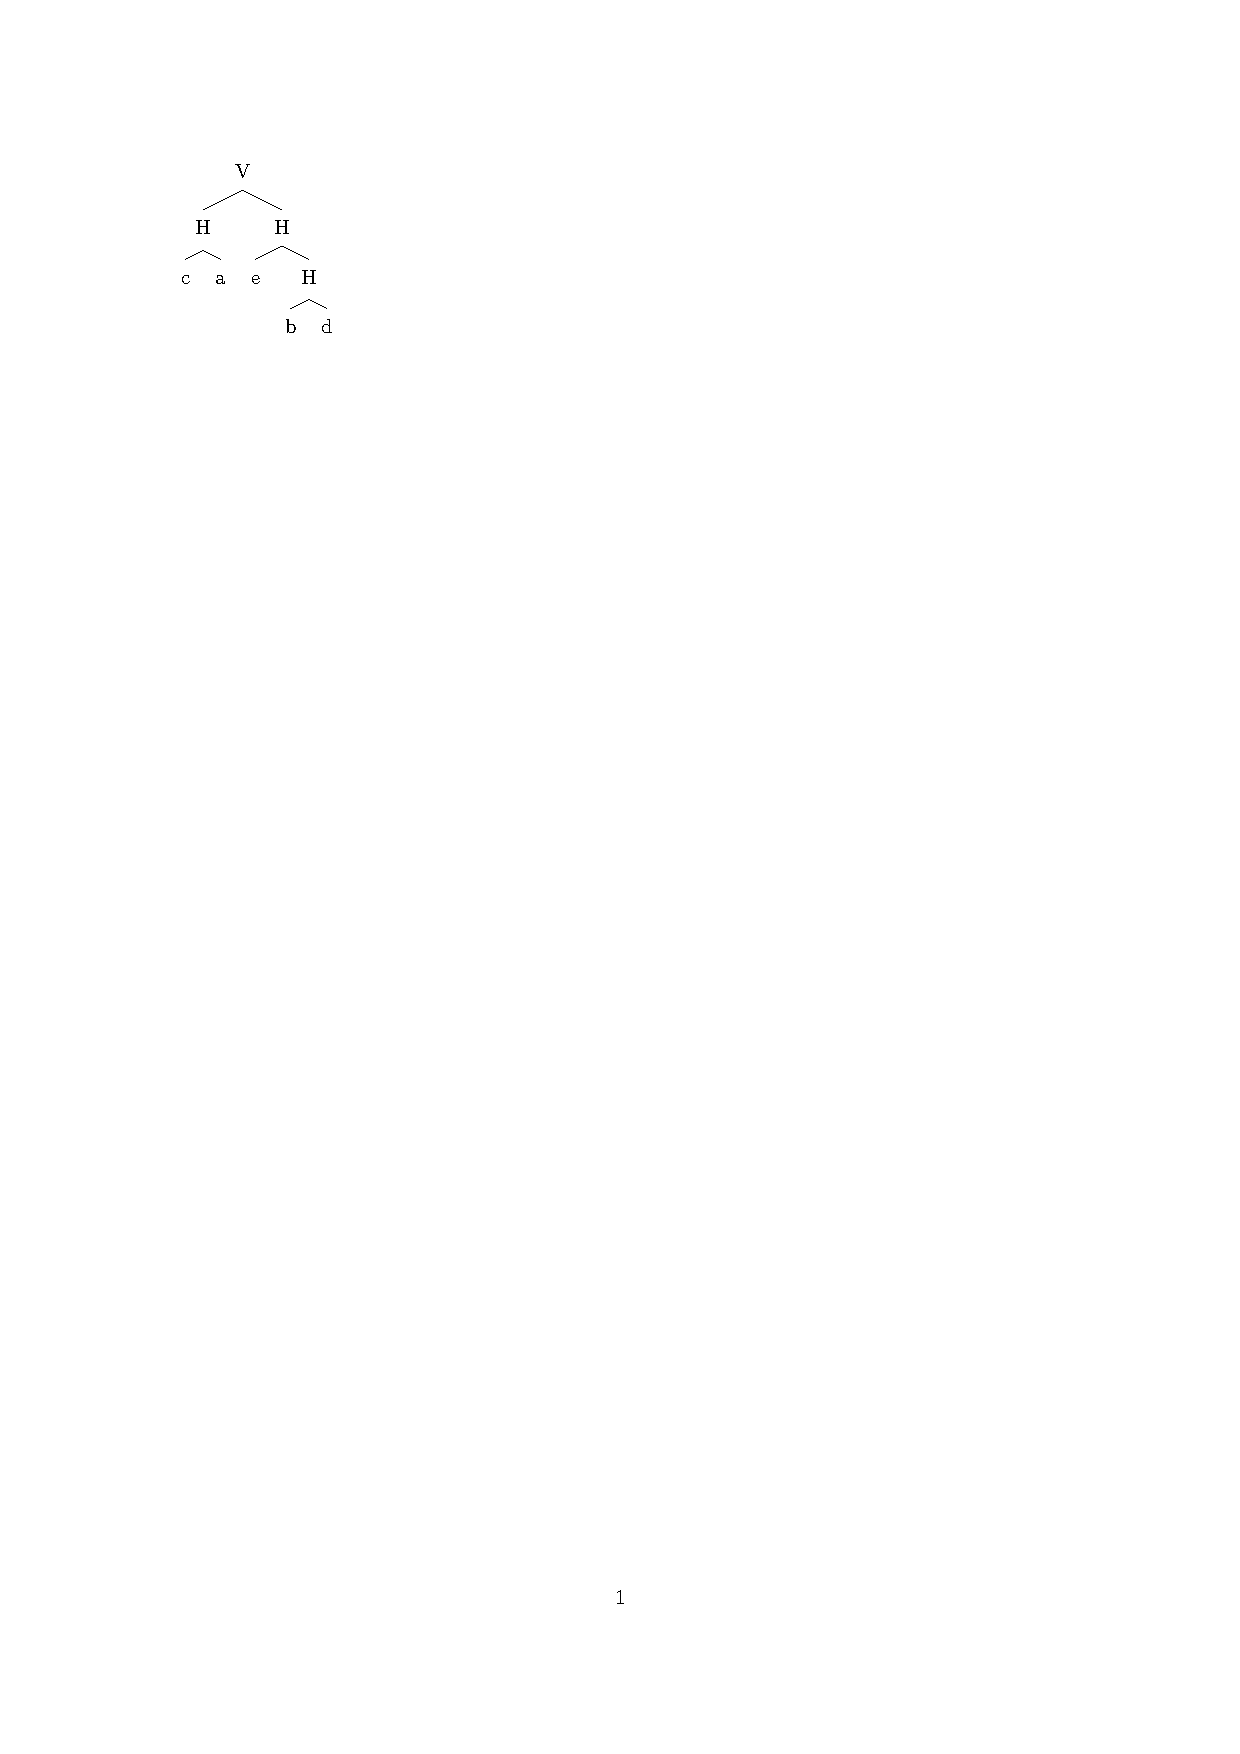
\includegraphics[trim=50 670 400 75,clip,width=1\linewidth]{tree2.pdf}
        \caption{New floorplan tree}
        \label{}
    \end{subfigure}
    \hspace{10mm}
    \begin{subfigure}{0.35\textwidth}
        \centering
        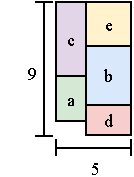
\includegraphics[trim=13 0 0 0,clip,width=0.6\linewidth]{3_floorplan2.pdf}
        \caption{New floorplan and bounding box}
        \label{}
    \end{subfigure}
\end{figure}

\section{Sequence pairs}

{\color{statement} Calculate the coordinates of the modules in the floorplan represented by the following sequence pair: (ABDECF, CBAEFD). }

First I drew the vertical and horizontal constraint graphs of the sequence pair to detect the critical (largest) paths.

\begin{figure}[H]
    \centering
    \begin{subfigure}{0.4\textwidth}
        \centering
        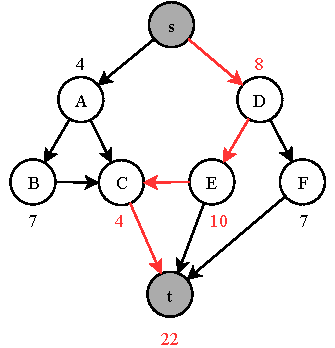
\includegraphics[width=1\linewidth]{4_vcg.pdf}
        \caption{VCG}
        \label{}
    \end{subfigure}
    \hfill
    \begin{subfigure}{0.47\textwidth}
        \centering
        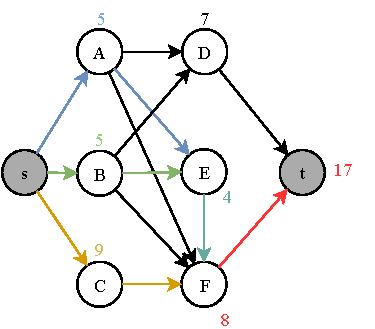
\includegraphics[width=1\linewidth]{4_hcg.pdf}
        \caption{HCG}
        \label{}
    \end{subfigure}
\end{figure}

With it, I was able to compute the bounding box and draw the floorplan (figure \ref{fig:f1}).

{\color{statement} Given the same sequence pair, and assuming that modules can be rotated 90º, propose some rotation to reduce the area.}

Rotating modules D, E and F, I obtained a smaller floorplan (figure \ref{fig:f2}) (probably the minimum with this sequence pair). I rotated modules that were in one of the critical paths (vertical or horizontal), and that improved the floorplan.

\begin{figure}[H]
    \centering
    \begin{subfigure}{0.3\textwidth}
        \centering
        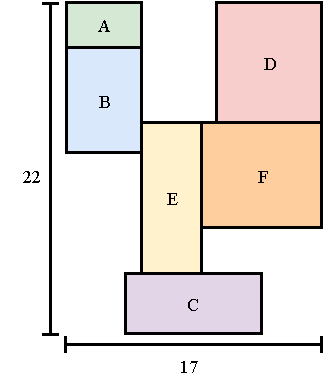
\includegraphics[width=1\linewidth]{4_1.pdf}
        \caption{Initial}
        \label{fig:f1}
    \end{subfigure}
    \hfill
    \begin{subfigure}{0.45\textwidth}
        \centering
        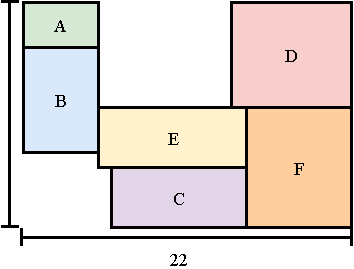
\includegraphics[width=1\linewidth]{4_2.pdf}
        \caption{With rotations}
        \label{fig:f2}
    \end{subfigure}
    \caption{Floorplans}
\end{figure}

\section{Partitioning}

{\color{statement} Given the graph in the figure, apply Kernighan\&Lin to find a good bi-partition, starting from the one in the figure. Show all the steps performed during the execution of the algorithm.}

Next you can see the two iterations that I had to do to reach the good bi-partition. Graph marked in grey is the best bi-partitioned graph of the iteration. The black border of the nodes means that they are fixed, i.e. they have already been switched.

\begin{figure}[H]
    \centering
    \begin{subfigure}{0.19\textwidth}
        \centering
        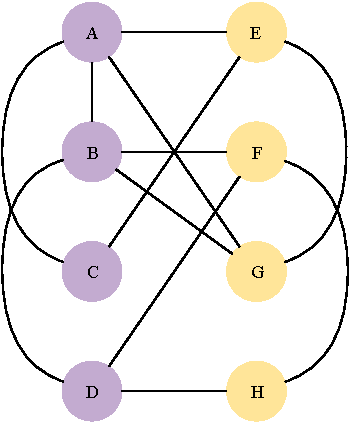
\includegraphics[width=1\linewidth]{5_11.pdf}
    \end{subfigure}
    \hfill
    \begin{subfigure}{0.19\textwidth}
        \centering
        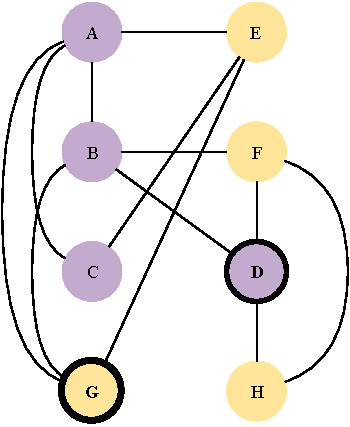
\includegraphics[width=1\linewidth]{5_12.pdf}
    \end{subfigure}
    \hfill
    \begin{subfigure}{0.19\textwidth}
        \centering
        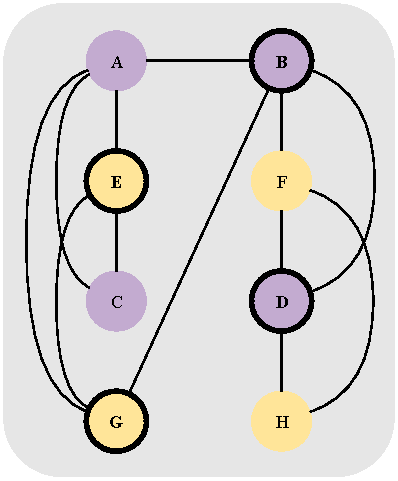
\includegraphics[width=1\linewidth]{5_13.pdf}
    \end{subfigure}
    \hfill
    \begin{subfigure}{0.19\textwidth}
        \centering
        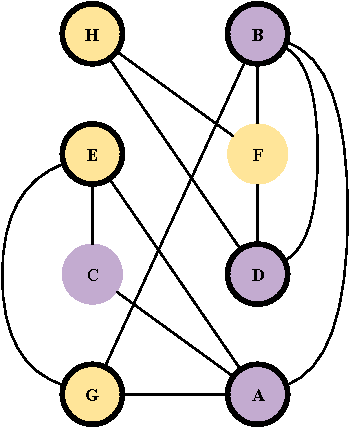
\includegraphics[width=1\linewidth]{5_14.pdf}
    \end{subfigure}
    \hfill
    \begin{subfigure}{0.19\textwidth}
        \centering
        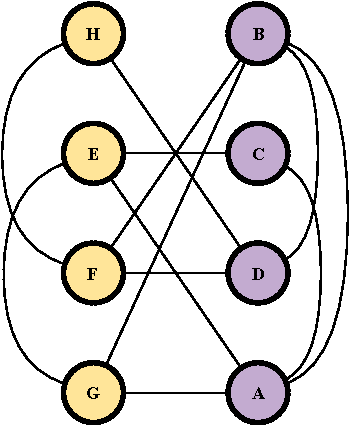
\includegraphics[width=1\linewidth]{5_15.pdf}
    \end{subfigure}
    \caption{First iteration of the algorithm.}
\end{figure}
\begin{figure}[H]
    \centering
    \begin{subfigure}{0.19\textwidth}
        \centering
        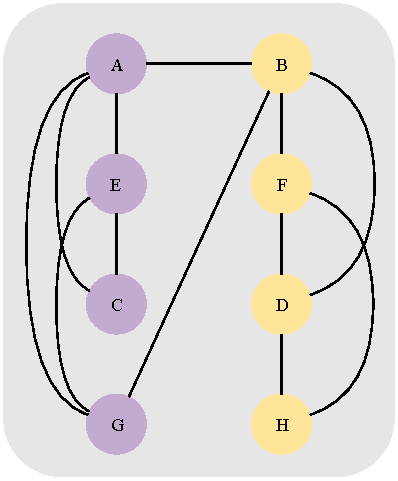
\includegraphics[width=1\linewidth]{5_21.pdf}
    \end{subfigure}
    \hfill
    \begin{subfigure}{0.19\textwidth}
        \centering
        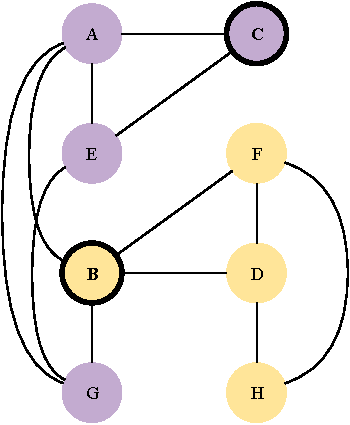
\includegraphics[width=1\linewidth]{5_22.pdf}
    \end{subfigure}
    \hfill
    \begin{subfigure}{0.19\textwidth}
        \centering
        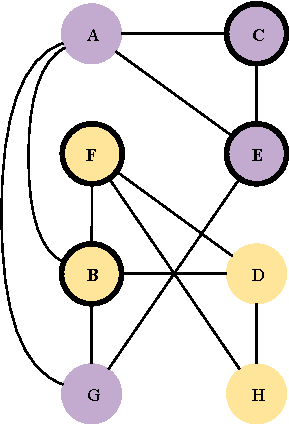
\includegraphics[width=1\linewidth]{5_23.pdf}
    \end{subfigure}
    \hfill
    \begin{subfigure}{0.19\textwidth}
        \centering
        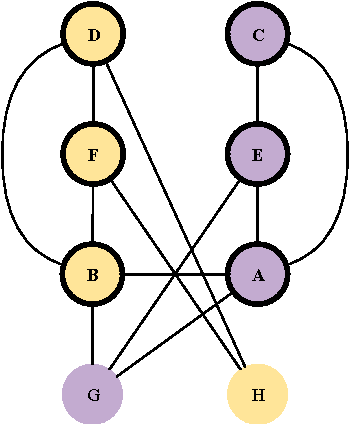
\includegraphics[width=1\linewidth]{5_24.pdf}
    \end{subfigure}
    \hfill
    \begin{subfigure}{0.19\textwidth}
        \centering
        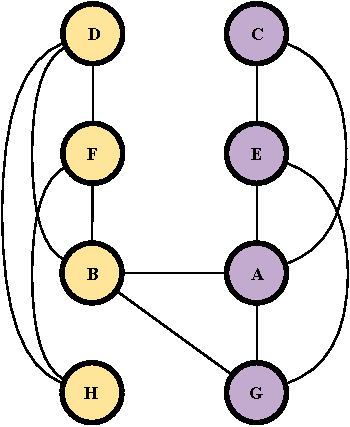
\includegraphics[width=1\linewidth]{5_25.pdf}
    \end{subfigure}
    \caption{Second iteration of the algorithm.}
\end{figure}


\end{document}